\section{Módulo de Optimización de Tiempos Semafóricos}
\label{sec:algoritmos_traffic_sync}

El módulo \texttt{traffic-sync} implementa el servicio de optimización de tráfico del sistema, exponiendo una API que recibe mediciones macroscópicas de tráfico por semáforo y devuelve configuraciones de tiempos optimizadas. Para ello combina dos componentes principales: un sistema de inferencia difusa tipo Mamdani, que evalúa el nivel de congestión a partir de variables de flujo, velocidad y densidad; y un algoritmo de optimización Particle Swarm Optimization (PSO), que ajusta dinámicamente los tiempos de verde con el objetivo de reducir la congestión estimada \cite{mamdani1975experiment,zadeh1965fuzzy,kennedy1995particle}.

% -----------------------------------------------------------------------------
\subsection{Lógica Difusa Mamdani}
\label{subsec:fuzzy_traffic_sync}

La lógica difusa proporciona un marco formal para representar razonamiento humano impreciso mediante variables lingüísticas y conjuntos difusos con grados de pertenencia entre 0 y 1 \cite{zadeh1965fuzzy,zadeh1971similarity}. En un sistema de inferencia Mamdani, las reglas tienen la forma ``SI condición ENTONCES acción'', donde tanto antecedentes como consecuentes se modelan como conjuntos difusos, y la salida final se obtiene tras un proceso de agregación y defuzzificación \cite{mamdani1975experiment,ross2010fuzzy}. Este enfoque resulta especialmente adecuado para describir estados de tráfico como ``flujo libre'', ``denso'' o ``congestionado'' a partir de variables macroscópicas continuas \cite{erdinc2023application,musriroh2020application}.

La Figura~\ref{fig:fuzzy_velocidad} ilustra un ejemplo de variable lingüística para velocidad promedio con tres términos (baja, media, alta) definidos mediante funciones de membresía, mostrando cómo un mismo valor numérico puede tener diferentes grados de pertenencia a múltiples categorías lingüísticas.

\begin{figure}[htbp]
\centering
\shorthandoff{>}
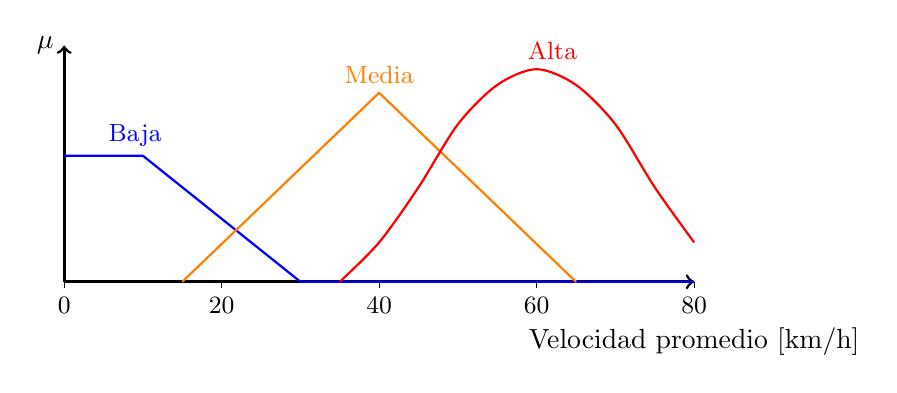
\begin{tikzpicture}[scale=1.0]
    % Ejes
    \draw[->,line width=1pt] (0,0) -- (8,0) node[below,yshift=-0.45cm] {Velocidad promedio [km/h]};
    \draw[->,line width=1pt] (0,0) -- (0,3.0) node[left] {$\mu$};

    % Marcas en eje x
    \foreach \x/\label in {0/0,2/20,4/40,6/60,8/80} {
        \draw (\x,0) -- (\x,-0.08) node[below] {\small \label};
    }

    % Baja: trapezoidal
    \draw[thick,blue]
        (0,1.6) -- (1,1.6) -- (3,0) -- (8,0);
    \node[blue,above] at (0.9,1.6) {\small Baja};

    % Media: triangular
    \draw[thick,orange]
        (1.5,0) -- (4,2.4) -- (6.5,0);
    \node[orange,above] at (4,2.4) {\small Media};

    % Alta: gaussiana aproximada
    \draw[thick,red,smooth] plot coordinates
        {(3.5,0) (4.0,0.5) (4.5,1.2) (5.0,2.0) (5.5,2.5) (6.0,2.7)
         (6.5,2.5) (7.0,2.0) (7.5,1.2) (8.0,0.5)};
    \node[red,above] at (6.2,2.7) {\small Alta};
\end{tikzpicture}
\shorthandon{>}
\caption{Variable lingüística \emph{velocidad promedio} con tres conjuntos difusos modelados mediante funciones de membresía trapezoidal, triangular y aproximadamente gaussiana \cite{ross2010fuzzy}.}
\label{fig:fuzzy_velocidad}
\end{figure}

En \texttt{traffic-sync}, el sistema de inferencia difusa se implementa en el módulo de lógica difusa, que está compuesto principalmente por el módulo de definición del sistema y el módulo de evaluación. El módulo de definición del sistema define las variables lingüísticas de entrada (por ejemplo, vehículos por minuto, velocidad media, tiempo medio de circulación, densidad) y la variable de salida asociada al nivel de congestión, junto con sus funciones de membresía triangulares y trapezoidales calibradas en base a datos de tráfico y criterios de ingeniería \cite{ross2010fuzzy,erdinc2023application}. La base de reglas Mamdani captura relaciones cualitativas del tipo ``SI flujo es alto Y velocidad es baja ENTONCES congestión es severa'', que reflejan tanto conocimiento experto como patrones observados en los datos \cite{musriroh2020application}.

La Figura~\ref{fig:mamdani_flujo} resume el flujo de procesamiento en un sistema de inferencia Mamdani aplicado al problema de congestión vehicular, mostrando las etapas desde la fuzzificación de entradas hasta la defuzzificación que produce el nivel de congestión final.

\begin{figure}[htbp]
\centering
\shorthandoff{>}
\begin{tikzpicture}[node distance=1.2cm,>=latex]

    \tikzstyle{block} = [rectangle, draw, rounded corners,
                         text width=5cm, align=center,
                         minimum height=0.9cm, font=\small]
    \tikzstyle{line} = [draw,->]

    \node[block] (inputs) {Entradas \emph{crisp}:\\ velocidad promedio, densidad, flujo};
    \node[block, below=of inputs] (fuzz) {Fuzzificaci\'on:\\ c\'alculo de grados de pertenencia};
    \node[block, below=of fuzz] (rules) {Base de reglas Mamdani:\\ combinaci\'on de etiquetas ling\"u\'isticas};
    \node[block, below=of rules] (agg) {Agregaci\'on:\\ unificaci\'on de salidas difusas};
    \node[block, below=of agg] (defuzz) {Defuzzificaci\'on:\\ c\'alculo de nivel de congesti\'on \emph{crisp}};
    \node[block, below=of defuzz] (output) {Salida:\\ nivel de congesti\'on num\'erico y categ\'orico};

    \path[line] (inputs) -- (fuzz);
    \path[line] (fuzz) -- (rules);
    \path[line] (rules) -- (agg);
    \path[line] (agg) -- (defuzz);
    \path[line] (defuzz) -- (output);

\end{tikzpicture}
\shorthandon{>}
\caption{Etapas principales de un sistema de inferencia difusa tipo Mamdani aplicado a congestión vehicular \cite{mamdani1975experiment,izquierdo2018mamdani}.}
\label{fig:mamdani_flujo}
\end{figure}

El módulo de evaluación expone funciones de alto nivel que reciben vectores de métricas de tráfico en formato estructurado y devuelven, para cada sensor o semáforo, un valor numérico de congestión y su categoría lingüística asociada. Estas funciones se utilizan en el pipeline principal del servicio web: el punto de entrada \texttt{/evaluate} recibe un lote de sensores, construye las entradas para el sistema difuso, ejecuta la evaluación Mamdani sobre cada uno y genera un conjunto de salidas que se utilizarán como insumo para la etapa de optimización PSO. De esta forma, la lógica difusa actúa como módulo de evaluación de desempeño que transforma mediciones de tráfico en un índice de congestión interpretable, que el optimizador buscará reducir.

% -----------------------------------------------------------------------------
\subsection{Optimización de Enjambre de Partículas (PSO)}
\label{subsec:pso_traffic_sync}

Optimización de Enjambre de Partículas (PSO) es un algoritmo de optimización metaheurística inspirado en el comportamiento colectivo de bandadas de aves y bancos de peces, en el que un conjunto de partículas explora el espacio de búsqueda guiado por su mejor experiencia individual y la mejor experiencia global del grupo \cite{kennedy1995particle,eberhart1995new}. Cada partícula representa una solución candidata (en este caso, una posible asignación de tiempo de verde para un grupo de semáforos) y actualiza su posición combinando tres componentes: inercia, atracción hacia su mejor posición personal y atracción hacia la mejor posición global conocida, ponderadas por parámetros que controlan el equilibrio entre exploración y explotación \cite{clerc2002particle,shi1998parameter}.

La Figura~\ref{fig:pso_enjambre} ilustra esquemáticamente el concepto del enjambre PSO en un espacio de búsqueda bidimensional, mostrando cómo las partículas se mueven influenciadas por su mejor experiencia personal ($p_i$) y la mejor experiencia global del grupo ($g$).

\begin{figure}[htbp]
    \centering
    \shorthandoff{>}
    \begin{tikzpicture}[scale=1.8]
        % Ejes
        \draw[->,line width=1.3pt] (-0.2,0) -- (6.2,0) node[below,font=\Large] {$x_1$};
        \draw[->,line width=1.3pt] (0,-0.2) -- (0,4.2) node[left,font=\Large] {$x_2$};
        
        % Partículas
        \fill[red] (1.0,3.0) circle (2.5pt) node[above left,font=\large] {$\mathbf{x}_1$};
        \fill[red] (2.0,2.5) circle (2.5pt) node[above,font=\large] {$\mathbf{x}_2$};
        \fill[red] (4.5,2.2) circle (2.5pt) node[above right,font=\large] {$\mathbf{x}_3$};
        
        % Mejor personal de una partícula
        \fill[orange] (1.8,3.4) circle (2.5pt) node[above,font=\large] {$p_1$};
        \draw[->,orange,dashed,line width=1.8pt] (1.0,3.0) -- (1.8,3.4);
        
        % Mejor global
        \fill[green!70!black] (3.0,1.6) circle (3pt) node[below right,font=\large] {$g$};
        \draw[->,green!70!black,dashed,line width=1.8pt] (2.0,2.5) -- (3.0,1.6);
        \draw[->,green!70!black,dashed,line width=1.8pt] (4.5,2.2) -- (3.0,1.6);
        
        % Leyenda
        \node[draw,fill=white,anchor=west] at (6.5,2.0) {%
          \begin{tabular}{@{}l@{}}
            \textcolor{red}{$\bullet$} Partículas (soluciones)\\
            \textcolor{orange}{$\bullet$} Mejor personal $p_i$\\
            \textcolor{green!70!black}{$\bullet$} Mejor global $g$
          \end{tabular}
        };
    \end{tikzpicture}
    \shorthandon{>}
    \caption{Esquema conceptual del enjambre PSO en un espacio de búsqueda bidimensional \cite{kennedy1995particle}.}
    \label{fig:pso_enjambre}
\end{figure}

En el módulo \texttt{traffic-sync}, la lógica de PSO se implementa en el módulo de optimización por enjambre de partículas, que incluye el módulo de función de aptitud y el módulo de optimización. El módulo de optimización define la función principal de PSO, que recibe información agregada de tráfico por grupo (clúster) y aplica PSO para determinar el tiempo de verde óptimo por grupo. Cada partícula codifica un tiempo de verde propuesto para el ciclo semafórico, inicializado alrededor de un valor base calculado mediante fórmulas clásicas de ingeniería de tráfico (función de cálculo de tiempo de verde en el módulo de aptitud), y restringido por límites mínimos y máximos coherentes con la normativa \cite{webster1958traffic,garber2019traffic}. El algoritmo utiliza configuraciones típicas de PSO (número de partículas, peso de inercia, componentes cognitiva y social, límites de velocidad) y añade mecanismos prácticos como parada temprana y reinicios parciales para evitar estancamiento en óptimos locales pobres.

La función de aptitud evalúa cada propuesta de tiempo de verde combinando la lógica difusa y las métricas de tráfico: dado un tiempo de verde candidato, recalcula métricas derivadas (como volumen efectivo, velocidad y densidad ajustadas) y vuelve a evaluar el nivel de congestión mediante el sistema Mamdani, obteniendo un valor numérico que se utiliza como medida a minimizar \cite{papageorgiou2003review,stevanovic2010adaptive}. De este modo, PSO busca explícitamente reducir el índice de congestión proporcionado por el módulo difuso, en lugar de optimizar una función analítica cerrada.

En el pipeline de \texttt{traffic-sync}, orquestado por la función principal del servicio web, el flujo es el siguiente: (i) el servicio recibe un lote de sensores en la API \texttt{/evaluate}; (ii) las mediciones se pasan al módulo difuso para obtener un nivel de congestión por sensor; (iii) se agrupan sensores con características similares (agrupamiento jerárquico), produciendo un conjunto de grupos de tráfico; (iv) se construye un conjunto de datos por grupo con métricas agregadas (por ejemplo, vehículos por minuto, velocidad media, densidad media, categoría de congestión); y (v) se aplica la función de optimización PSO sobre estos grupos para obtener tiempos de verde optimizados por grupo. La respuesta de la API se construye como un lote de optimizaciones, donde cada entrada incluye el tiempo de verde recomendado, el tiempo de rojo derivado, el nivel de congestión original y optimizado, y las categorías lingüísticas correspondientes, preparados para su consumo posterior por el módulo de control de semáforos y por el módulo de almacenamiento.

En conjunto, la integración entre lógica difusa Mamdani y PSO en \texttt{traffic-sync} permite que la optimización de tiempos semafóricos se base en una medida de congestión que captura adecuadamente la percepción y el comportamiento del tráfico urbano, mientras que el metaheurístico proporciona un mecanismo flexible para ajustar los parámetros de control en escenarios donde la función objetivo no es derivable y debe evaluarse a través de simulación o reglas de inferencia \cite{ross2010fuzzy,poli2007particle}.

La Figura~\ref{fig:sync_architecture} ilustra la arquitectura general del módulo \texttt{traffic-sync}, mostrando la interacción entre los componentes de lógica difusa y PSO, así como el flujo de datos desde la recepción de métricas de tráfico hasta la generación de configuraciones optimizadas de tiempos semafóricos.

\begin{figure}[htbp]
\centering
\shorthandoff{>}
\begin{tikzpicture}[
    node distance=1.3cm,
    block/.style={rectangle, draw, rounded corners, fill=blue!10,
                  text width=3cm, align=center, minimum height=1cm},
    data/.style={rectangle, draw, fill=yellow!10,
                 text width=2.5cm, align=center, minimum height=0.7cm},
    arrow/.style={->,thick,>=stealth}
]

    % Entrada
    \node[data] (input) {Métricas de\\tráfico};
    
    % Lógica difusa
    \node[block, below=of input] (fuzzy) {Sistema Difuso\\Mamdani};
    \node[data, below=of fuzzy] (congestion) {Nivel de\\congestión};
    
    % Agrupamiento
    \node[block, right=2.5cm of fuzzy] (clustering) {Agrupamiento\\jerárquico};
    
    % PSO
    \node[block, below=of clustering] (pso) {Optimización\\PSO};
    
    % Función de aptitud
    \node[block, left=2.5cm of pso] (fitness) {Función de\\aptitud};
    
    % Salida
    \node[data, below=of pso] (output) {Tiempos\\optimizados};
    
    % Flechas
    \draw[arrow] (input) -- (fuzzy);
    \draw[arrow] (fuzzy) -- (congestion);
    \draw[arrow] (congestion) -- (clustering);
    \draw[arrow] (clustering) -- (pso);
    \draw[arrow] (pso) -- (output);
    \draw[arrow, dashed] (pso) -- (fitness);
    \draw[arrow, dashed] (fitness) -- node[left,font=\scriptsize] {evaluar} (fuzzy);

\end{tikzpicture}
\shorthandon{>}
\caption{Arquitectura del módulo \texttt{traffic-sync} integrando lógica difusa Mamdani y optimización PSO.}
\label{fig:sync_architecture}
\end{figure}

